%% --------------------------------------------------------------------------
\subsection{In-Memory Graph Analytics}
\label{sec:eval:inmem}

% Workload: GAPBS kernels -- PageRank, BFS, CC, SSSP, Triangle Counting.
% Competitors: GAPBS (native CSR), Ligra.
% Graphs: cit-Patents, twitter_mpi, kronecker-26.
%
% Key argument: algorithm time alone is slower than GAPBS (expected -- CSR is
% purpose-built), but total time including preprocessing/load is competitive
% because \project{} avoids a separate graph-loading step.
%
% Include table: algo time, preprocessing time, total time for each system x kernel.
We create Docker containers for each system, restricting each to one NUMA node (96 threads) with local memory; all cores in the node are used for analytics.
For every system, we measure the preprocessing time to convert an edge list into the system's in-memory format.
We then measure the total time to run the four graph kernels that all four systems implement: PageRank, Connected Components, BFS, and Betweenness Centrality.

%%%%%%%%%%%%%%%%%%%%%%%%%%%%%%%%%%%%%%%%%%%%%%%%%%%%%%%%%%%%%%%%%%%%%%%%%%%%%%%%
\begin{figure}[t]
  \centering
  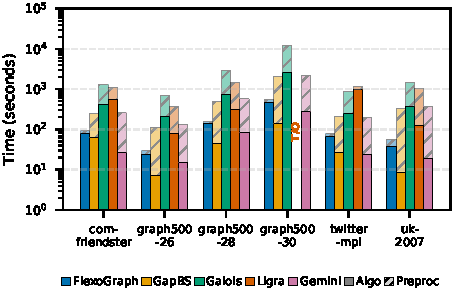
\includegraphics[width=\columnwidth]{content/fig/in-mem/flexograph_inmem_results.pdf}
  \caption{In-memory graph analytics performance. The hatched portions of each bar show the preprocessing time.\PM{add error bars}}
  \label{fig:inmem-results}
\end{figure}
%%%%%%%%%%%%%%%%%%%%%%%%%%%%%%%%%%%%%%%%%%%%%%%%%%%%%%%%%%%%%%%%%%%%%%%%%%%%%%%%
\autoref{fig:inmem-results} shows the results.
For this experiment, we used the analytics-friendly adjacency list layout for \project{} and opened the \wt{} connection with \texttt{mmap\_all=true,cache=800GB}, mapping data files directly into the process address space with an 800\,GB cache, much larger than the working set for any analytics kernel.
%%%%%%%%%%%%%%%%%%%%%%%%%%%%%%%%%%%%%%%%%%%%%%%%%%%%%%%%%%%%%%%%%%%%%%%%%%%%%%%%
\begin{table}[h]
  \centering
  \small
  \begin{tabular}{lrrrrr}
    \toprule
    Dataset & FG:Adj & GapBS & Galois & Ligra & Gemini \\
    \midrule
    com-friendster & 34.55 & 30.10 & 36.46 & 118.52 & 19.97 \\
    graph500-26 & 20.50 & 17.35 & 24.38 & 68.21 & 11.20 \\
    graph500-28 & 80.57 & 70.06 & 75.13& 287.19 & 44.71 \\
    graph500-30 & 322.29 & 281.58 & 283.67 & OOM & 178.55 \\
    twitter-mpi & 25.39 & 31.34 & 23.12 & 118.66 & 18.15 \\
    uk-2007 & 60.95 & 51.88 & 58.42 & 210.48 & 31.48 \\
    \bottomrule
  \end{tabular}
  \caption{Peak memory usage (GiB) of in-memory systems. \PM{I will fill in the missing numbers.}}
  \label{tab:inmem-memory}
\end{table}
%%%%%%%%%%%%%%%%%%%%%%%%%%%%%%%%%%%%%%%%%%%%%%%%%%%%%%%%%%%%%%%%%%%%%%%%%%%%%%%%
We measure the combined runtime to execute \mbox{graphalytics} kernels (solid bars in \autoref{fig:inmem-results}) and the peak memory usage for all in-memory systems during analytics kernel execution (\autoref{tab:inmem-memory}).
\project{} outperforms both Galois and Ligra on every dimension: faster algorithmic runtime, faster preprocessing, and lower memory consumption.
Ligra consistently uses $\approx$3$\times$ the graph size in memory, so the Linux OOM killer terminates it on graph500-30.
The comparison with GapBS and Gemini is more nuanced.
Both outperform \project{} on kernel runtime alone. However, when even a single ingest time for the four kernels is included, \project{} is faster, and ingest is the normal operating mode for these systems.
Gemini uses the least memory of all systems on every graph.
GapBS is also relatively memory efficient consuming less memory than \project{} on five of the six graphs \PM{find these missing memory numbers}.

\textbf{Takeaway}: \project{} avoids costly ETL thanks to its ability to run directly on a persistent representation.
This benefit comes at slightly increased memory consumption relative to the lightest competitors and decreased performance if the other systems are able to retain an in-memory representation.
\PM{insert the edge-key numbers}

\PM{we need ekey vs adj list numbers here. This is covered in the Graphalytics comparison on dynamic in-mem systems. }
